\section{Full governing equation for vertically isothermal disks in
  the vertically global shearing box}\label{adia_improve}
Here we explain the derivation of Eq. \ref{vertiso_gov} used in our 
analytical discussion in \S\ref{analytical}. We shall need the
vertical derivative of the epicyclic frequency $\kappa$. In the global
disk with $\Gamma=1$ we have 
\begin{align}\label{dkappa2}
  \frac{\p\kappa^2}{\p z} = 4 \frac{\p\Omega^2}{\p z} + r\frac{\p}{\p
    r}\frac{\p\Omega^2}{\p z} = -
  \frac{\p\ln\rho}{\p z}\frac{qc_s^2}{r^2} \left(
    \frac{3z^2}{r^2+z^2}-1\right) \equiv - \frac{\p\ln\rho}{\p z}\frac{qc_s^2}{r^2}F(r,z).
\end{align}
% For the local problem we may then write
% \begin{align}
%   \frac{dD}{dz}  = - \frac{d\ln\rho}{dz}\frac{qc_s^2}{r^2}F(z),
% \end{align}
The function $F$ increases monotonically from $F=-1$ at $z=0$ to $F\to2$
as $|z|\to\infty $, so $|F|=O(1)$. 

In the vertically global shearing box (VGSB) approximation, we set
$\hat{g}_c=0$ in Eq. \ref{lin_mass} --- \ref{lin_energy}. We then eliminate
the horizonatal velocity perturbations ($\delta v_x,\, \delta v_y$) to
obtain  
%we can eliminate variables 
%to obtain a pair or ordinary differential
%equations for $W,Q$ as 
\begin{align}
  & \ii\sigma\delta v_z = \frac{dW}{dz} + \frac{d\ln{\rho}}{d z}\left(W-Q\right),\label{ode_vz} \\
  &\frac{\sigma^2}{c_s^2}Q + \frac{\sigma^2k_x^2}{D}W =\ii\sigma \left(\frac{\ii
      k_x r}{D}\frac{d\Omega^2}{dz} -
    \frac{d\ln{\rho}}{dz}\right)\delta v_z - \ii\sigma \frac{d\delta v_z}{dz},
  % \left[\frac{dW}{dz} + \frac{d\ln{\rho}}{dz}\left(W-Q\right)\right] 
  % \notag\\
  % &- \frac{d^2W}{dz^2} - \frac{d\ln{\rho}}{dz}\left(\frac{dW}{dz} -
  %   \frac{dQ}{dz}\right) - \frac{d^2\ln{\rho}}{dz^2}\left(W-Q\right),
  \label{ode_w}\\
%  &\sigma^2W - \frac{\gamma}{\Gamma}\sigma^2 Q +
%  \frac{\ii\sigma}{t_c}\left(W-\frac{Q}{\Gamma}\right) 
%  =\ii \sigma c_s^2\frac{d\ln{\rho}}{dz}\left(\frac{\gamma}{\Gamma} -
%    1\right)\delta v_z,  
  &\sigma^2W - \gamma\sigma^2 Q +
  \frac{\ii\sigma}{t_c}\left(W-Q\right) 
  =\ii \sigma c_s^2\frac{d\ln{\rho}}{dz}\left(\gamma -
    1\right)\delta v_z,
  % 
  % \left[\frac{dW}{dz} + \frac{d\ln{\rho}}{dz}\left(W-Q\right)\right],
  \label{ode_Q} 
\end{align}
(note that $\Gamma=1$ has been used) where
\begin{align}
  D \equiv \kappa^2 - \sigma^2,
\end{align} 
and we have replaced the notation $\p_z$ by $d/dz$ since we are
considering solutions at a fixed radius. 

% In \S\ref{approx_gov} we made the replacement $D\to\Omega_k^2$ before
% eliminating variables to obtain a single equation for $\delta v_z$ in
% vertically isothermal disks, Eq. \ref{vertiso_gov}.  
% This procedure ignores the vertical dependence of
% $D=\kappa^2(z) - \sigma^2$. We show here that this has no serious 
% consequence for thin disks. 

%For the radially local problem, we eliminate $W$ and $Q$ from Eq. \ref{ode_w}---\ref{ode_Q} and
%Eq. \ref{lin_vz}  (with $\Gamma=1$), but now retain the vertical dependence
%of $D$ using Eq. \ref{dkappa2}, to obtain  

We now eliminate $W,\, Q$ from Eq. \ref{ode_vz} --- \ref{ode_Q} in
favor of $\delta v_z$, making use of Eq. \ref{dkappa2} to evaluate
$dD/dz$, to obtain  

\begin{align}\label{full_ode}
  0 =& \frac{d^2\delta v_z}{dz^2} + \left[1 + \frac{\ii k_x c_s^2
      q}{Dr} - \frac{k_x^2c_s^2}{\left(k_x^2c_s^2 + \chi
        D\right)}\frac{qc_s^2F}{Dr^2}\right]\frac{d\ln\rho}{dz}\frac{d\delta
    v_z}{dz} \notag\\
  &+ \left\{\sigma^2\left(\frac{k_x^2}{D} +
      \frac{\chi}{c_s^2}\right) + \left(\chi + \frac{\ii k_x c_s^2
        q}{Dr}\right)\frac{d^2\ln\rho}{dz^2} -
    \frac{c_s^2}{D}\left(\frac{d\ln\rho}{dz}\right)^2\left(k_x^2 -
      \frac{\ii k_x q}{r}\right)
   \left[\left(1-\chi\right) +
     \frac{\chi}{\left(k_x^2c_s^2 + \chi D\right)}\frac{qc_s^2 F}{r^2}\right] 
   \right\}\delta v_z,
\end{align}
where we recall $\chi = \left(1-\ii\sigma t_c\right)/\left(1-\ii\sigma
t_c \gamma\right)$. Making the low frequency and Keplerian
approximations is equivalent to the replacement $D\to
\Omega_k^2$. This gives, in terms of dimensionless variables,  
\begin{align}
  &\delta v_z ^{\prime\prime} + \left[1 + \ii\epsilon q\hat{k} -
    \frac{ \hat{k}^2}{
      \left(\hat{k}^2+\chi\right)}q \epsilon^2F\right]\ln\rho^{\prime}\delta v_z^\prime +
  \left\{\left(\chi + \ii \epsilon q
      \hat{k}\right)\ln\rho^{\prime\prime} - \ln\rho^{\prime
      2}\left(\khat^2 -
      \ii\epsilon
      q\hat{k}\right)\left[1 - \chi +
      \frac{\chi}{\left(\hat{k}^2+\chi\right)}q\epsilon^2F\right]\right\}\delta v_z \notag\\&=
  -\hat{\sigma}^2\left(\hat{k}^2+\chi\right)\delta v_z\label{adia_diso3}.
\end{align} 
Since we are interested in thin disks with $\epsilon \ll 1$ and $|q| =
O(1)$, we neglect the terms proportional to $\epsilon^2$, which gives 
Eq. \ref{vertiso_gov_nondim} (the dimensional version being
Eq. \ref{vertiso_gov}). This is equivalent to neglecting the   
vertical dependence of $D$ by setting $D\to\Omega_k^2$ in
Eq. \ref{ode_w} before eliminating variables in favor of $\delta
v_z$, which is the simpler way to obtain Eq. \ref{vertiso_gov}. 

%Thus, a simpler route to the governing
%equation (Eq. )  

%Eq. \ref{adia_diso3} differs from Eq. \ref{vertiso_gov_nondim} by terms
%proportional to $\epsilon^2$. For a thin disk ($\epsilon\ll1$) with
%$|q|=O(1)$, as considered in this work, neglecting these terms has no
%qualitative effect on the discussion in \S\ref{analytic_relax}. 
% In deriving Eq. \ref{vertiso_gov}, the vertical dependence of
% $D=\kappa^2(z)-\sigma^2$ was ignored because the replacement
% $D\to\Omega_k^2$ was made before eliminating variables in favor of
% $\delta v_z$. In Appendix \ref{adia_improve} we show that making this
% replacement after eliminating variables, which involves $dD/dz$,
% introduces terms of $O(\epsilon^2)$. Since we are interested in 
% thin disks ($\epsilon\ll 1 $), e.g. protoplanetary disks where 
% $\epsilon\lesssim 0.1$ \citep{chiang10}, these terms introduce
% unnecessary complexity for the present discussion. 
      



\section{Applicability of the  VGSB}\label{global_corr}
%In \S\ref{analytical} we effectively employed the vertically global
%shearing box \citep[VGSB,][]{mcnally14} to make analytic progress. 
The vertically global shearing box \citep[VGSB,][]{mcnally14} is an
extension of the standard shearing box \citep[SSB,][]{goldreich65} to
background shear flows that are height dependent. 
%As in the SSB, in
%the VGSB the equilibrium disk structure is assumed to be homogeneous
%in the radial ($x$) direction.  
Within the VGSB framework, the vertical shear $d\Omega/dz$
can be freely specified. We choose $d\Omega/dz$ to be that due to the
radial temperature gradient in the global disk
(Eq. \ref{vertical_shear}). However, explicit dependencies on the
radial disk structure are ignored elsewhere in the linearized equations
as described below. We show in the following sections that this
inconsistency only becomes important in the adiabatic limit, which is
not the relevant regime for the VSI. 

%is only important when
%considering adiabatic limit, which is not the relevant regime for the
%VSI.  

The background radial disk structure explicitly appears 
in the linearized mass, radial momentum and energy equations
(Eq. \ref{lin_mass}, \ref{lin_vx} and \ref{lin_energy}) as the terms
proportional to $\hat{g}_c$. Nominally $\hat{g}_c=1$.      
In the VGSB (and SSB) these terms are neglected by setting
$\hat{g}_c=0$. For a power-law disk, these radial gradients  
are $O(r^{-1})$, and they appear in comparison with terms of
$O(k_x)$. The neglected terms therefore have a relative magnitude of
$O(\epsilon/\khat)$, which is small for thin disks ($\epsilon\ll1$)
and/or small radial wavelengths ($\khat\gg 1$). 
 


% The difference between the linear problem in the VGSB 
% and the radially-local approximation adopted in our numerical study
% is the absence of terms explicitly associated with the radial disk structure in
% the VGSB. 


%However, background radial gradient terms 
%are ignored elsewhere in the VGSB (which is done by setting
%$\hat{g}_c=0$).         
   
% \begin{align}
%   \ii \sigma W  &=c _s^2(r_0, z)\left( \left.\frac{\p\ln\rho}{\p
%       z}\right|_0 \delta v_z + \frac{\gamma}{\Gamma} \frac{d\delta
%     v_z}{dz}\right) + \left[\ii k_xc_s^2(r_0,z)
%   \frac{\gamma}{\Gamma} + \hat{g}_c\left.\frac{1}{\rho}\frac{\p P}{\p
%       r}\right|_0\right]\delta v_x  +
% \frac{1}{t_c}\left(W-\frac{Q}{\Gamma}\right),\label{gcorr_terms1}\\
% \ii \sigma Q &= c_s^2(r_0,z)\left(\ii k_x + \hat{g}_c
%   \left.\frac{\p\ln{\rho}}{\p r}\right|_0\right)\delta v_x + c _s^2(r_0, z)\left( \left.\frac{\p\ln\rho}{\p
%       z}\right|_0 \delta v_z + \frac{d\delta
%     v_z}{dz}\right),\label{gcorr_terms2} \\
% \ii \sigma \delta v_x & = \ii k_x W  -
% \hat{g}_c\frac{1}{c_s^2(r_0,z)}\left.\frac{1}{\rho}\frac{\p P}{\p
%   r}\right|_0Q - 2\Omega(r_0,z)\delta v_y,\label{gcorr_terms3}
% \end{align}
% where subscript $0$ denotes evaluation at $r=r_0$. We recall terms
% proportional to $\hat{g}_c$ are associated with the background density
% and pressure radial structures, and nominally $\hat{g}_c=1$.   

\subsection{Spurious growth of adiabatic perturbations in the VGSB}\label{analytic_adia} 
A limitation of the VGSB is that it cannot be used in the
adiabatic limit, even if the above conditions are satisfied. We explain this by considering vertically isothermal
disks and setting  $\beta\to\infty$ in 
Eq. \ref{vertiso_gov_nondim} % (which itself is obtained by setting
% $\hat{g}_c=0$ in Eq. \ref{lin_mass}---\ref{lin_energy})
to give 
\begin{align}
  0 =\dd v_z^{\prime\prime} + \left(1 + \ii \epsilon q
    \hat{k}\right)\left(\ln\rho^{\prime}\delta v_z\right)^\prime
  +\left\{\hat{\sigma}^2\left(\frac{1}{\gamma}+\hat{k}^2\right) 
    -\left(\frac{\gamma-1}{\gamma}\right)\left[\ln\rho^{\prime\prime}+\hat{k}^2\left(1-\frac{\ii\epsilon  
          q}{\hat{k}}\right)\ln\rho^{\prime 2}\right]\right\}\delta v_z.\label{adia_iso3}
\end{align}
We multiply Eq. \ref{adia_iso3} by $\rho\delta v_z^*$ and
integrate vertically, assume boundary terms vanish when integrating by
parts, to obtain
\begin{align}
  \hat{\sigma}^2\left(\frac{1}{\gamma} +
    \hat{k}^2\right)\int_{\zhat_1}^{\zhat_2}\rho|\delta
  v_z|^2 d\zhat 
  =&  \left(\frac{\gamma-1}{\gamma}\right)
  \int_{\zhat_1}^{\zhat_2}\rho|\delta v_z^\prime|^2 d\zhat
  +\frac{1}{\gamma}\int_{\zhat_1}^{\zhat_2}\frac{1}{\rho}|(\rho\delta
  v_z)^\prime|^2 d\zhat\notag\\
&+
  \left(\frac{\gamma-1}{\gamma}\right)\hat{k}^2\left(1-\frac{\ii\epsilon
      q}{\hat{k}}\right) \int_{\zhat_1}^{\zhat_2}\rho\ln\rho^{\prime
    2}|\delta v_z|^2 d\zhat
+ \ii\epsilon q \hat{k}
  \int_{\zhat_1}^{\zhat_2}\ln\rho^\prime(\rho\delta v_z^*)^\prime
  \delta v_z d\zhat.\label{adia_integral}
\end{align}
% When $q\equiv0$, all the terms on the right-hand-side (RHS) are real. Then
% $\hat{\sigma}^2$ is real, and  $\hat{\sigma}^2>0$ if $\gamma>1$. As
% expected, a sub-adiabatically stratified disk is stable in the absence
% of vertical shear. 
In the presence of vertical shear $q\neq0$, Eq. \ref{adia_integral}
suggests $\hat{\sigma}^2$ is complex for real $\khat$, which implies the
possibility of instability, regardless of the value of
$|\gamma-1|$. This is contradicts the second Solberg-Hoiland criterion 
(Eq. \ref{solberg2}), which imply instability for adiabatic
perturbations in a thin, vertically isothermal disk would require 
$|\gamma-1|\ll1$. 
%also need real freq^2 in adia limit 
This is because the VGSB retains the vertical shear
($\p_z\Omega$) from the global disk, but ignores the global radial
disk structure responsible for it. Nevertheless, we demonstrate below
that this inconsistency is unimportant for the VSI because it occurs
for $\beta\ll1$.   %and small scale

\subsection{Effect of global radial gradients}
In  Fig. \ref{gcorr_compare}, we plot the effect of the global radial gradient terms
proportional to $\hat{g}_c$ in Eq. \ref{lin_mass}---\ref{lin_energy}
by calculating the
fundamental VSI growth rates using three approaches. We compute growth rates from the dispersion
relation Eq. \ref{relax_disp}, which assumes $\hat{g}_c=0$;  from
Eq. \ref{lin_mass}---\ref{lin_energy} with $\hat{g}_c=0$; and from
Eq. \ref{lin_mass}---\ref{lin_energy}  with $\hat{g}_c=1$.   

All three methods give similar behavior, and growth rates are in close
agreement for $\beta\lesssim 1$. Differences arise for 
$\beta\gtrsim1$, and as $\beta\to\infty$ the VGSB framework gives a
(spurious) growth rate as expected from the discussion
above. Inclusion of the global radial gradient terms results in the
correct behavior  ($\nu\to0$ as $\beta\to\infty$). Despite this
caveat, Fig. \ref{gcorr_compare} shows that provided we consider
$\beta\ll1$, then the VGSB framework is adequate for studying the
VSI. 
  
\begin{figure}
  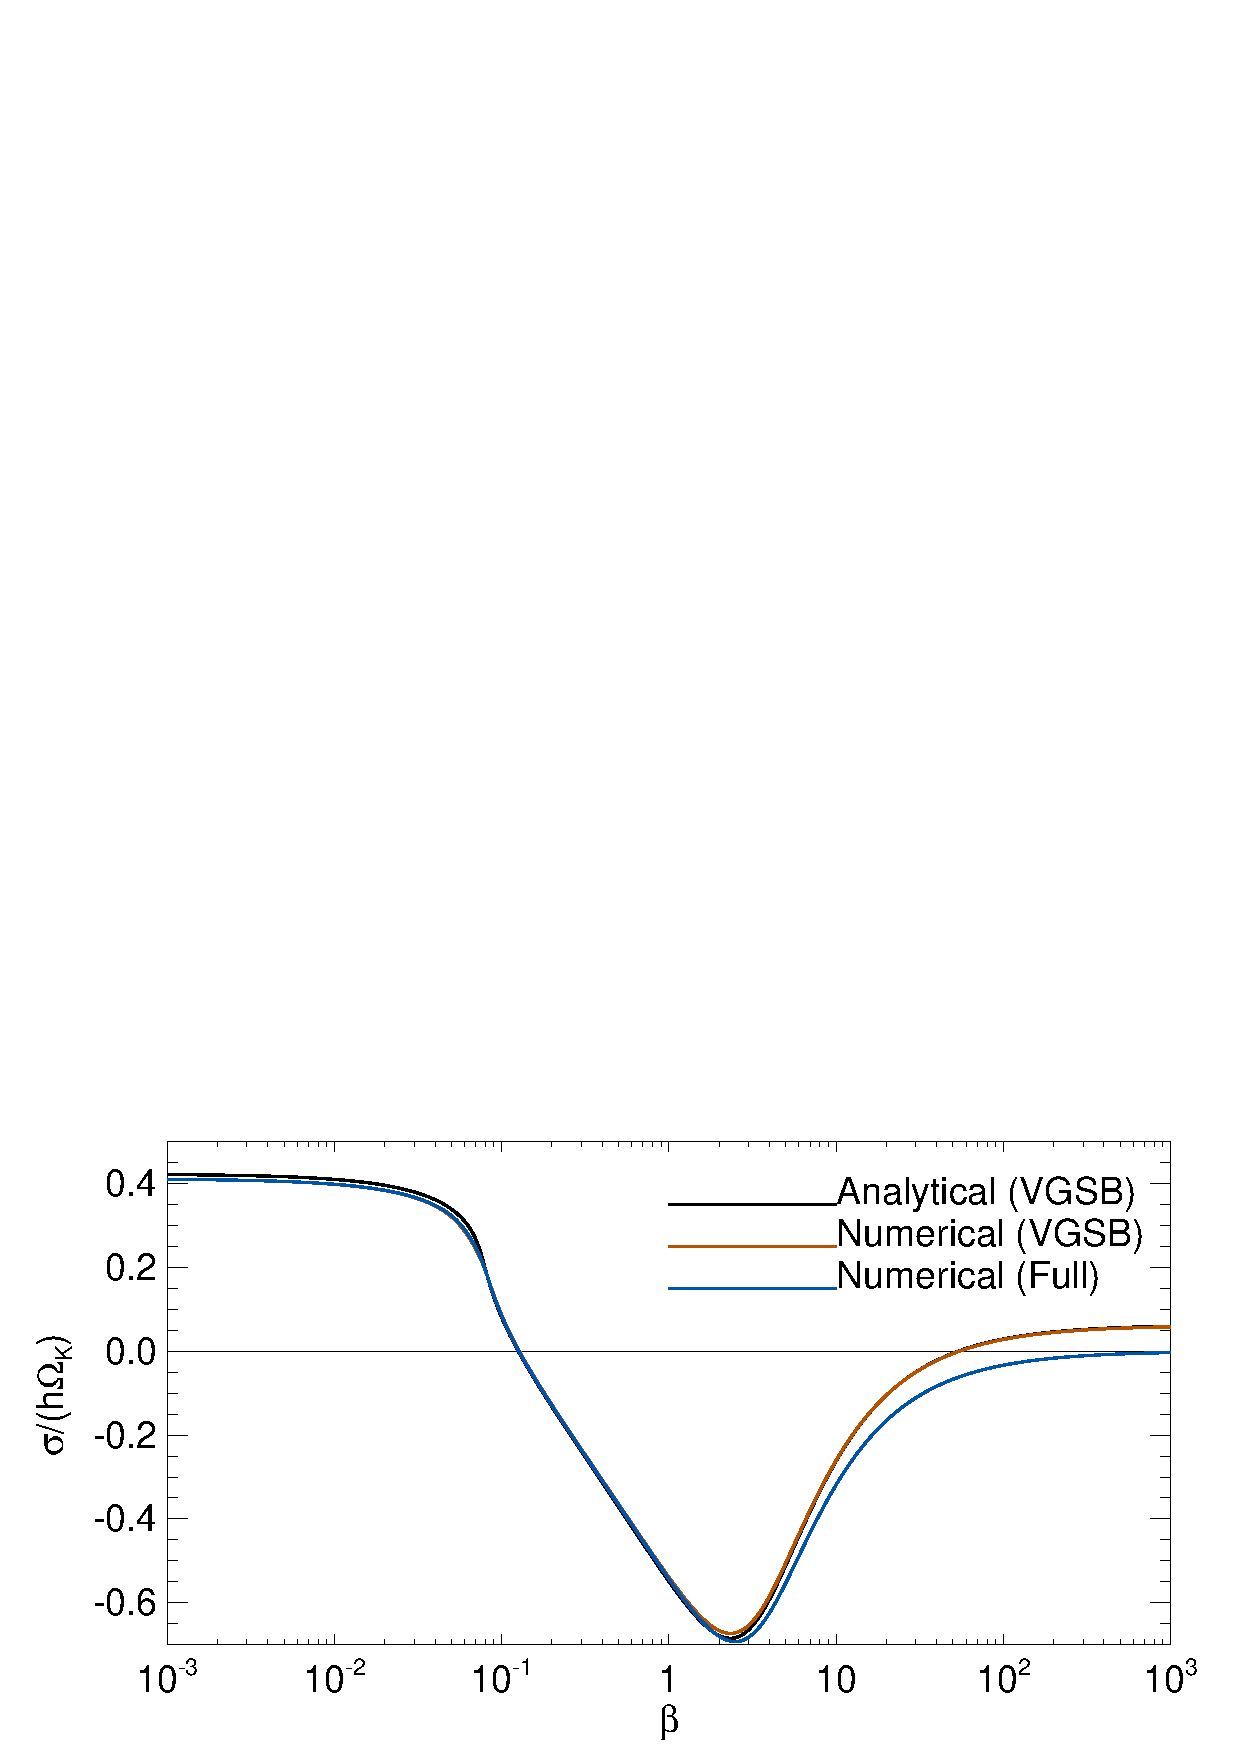
\includegraphics[width=\linewidth,clip=true,trim=0cm 0.0cm 0cm
  0cm]{figures/gcorr_compare} 
  \caption{Growth rate of the fundamental VSI mode as a function of
    the thermal relaxation time $\beta$. The `Analytical (VGSB)' curve
    is calculated from the dispersion relation Eq. \ref{relax_disp};
    the `Numerical (VGSB)' curve is obtained by numerically solving
    the linear problem, Eq. \ref{lin_mass}---\ref{lin_energy}, with $\hat{g}_c=0$
    (which defines the linear VGSB equations); and the `Numerical
    (Full)' curve is obtained by numerically solving 
    Eq. \ref{lin_mass}---\ref{lin_energy}  with $\hat{g}_c=1$, which
    accounts for the radial disk structure.  
    The disk parameters are $(\gamma, \Gamma)=(1.4, 1.011)$ and
    $(p,q,\epsilon)=(-1.5,-1,0.05)$. The perturbation
    wavenumber is $\khat=30$. 
    \label{gcorr_compare}}  
\end{figure}










\section{Linear problem in the isothermal limit}\label{iso_discuss}  
Here we summarize selected results for isothermal
perturbations ($\beta\equiv 0$) in vertically isothermal disks 
($\Gamma=1$) in the VGSB framework. In this case Eq. \ref{ode_Q}
becomes    
\begin{align} 
  Q = W 
\end{align}
(i.e. $\delta P = c_s^2\delta \rho$), and so $  \ii\hat{\sigma}c_s\delta v_z = W^\prime $
from Eq. \ref{lin_vz}. For isothermal perturbations it is 
simpler to work with an equation for $W$ by substituting $Q=W$ into
Eq. \ref{ode_w}. In this case, we shall not yet make the low frequency
approximation, but first make the  Keplerian approximation. We
obtain, in terms of dimensionless variables, 
\begin{align}
  0 = W^{\prime\prime} + \left[\ln\rho^\prime - \frac{\ii \epsilon q \hat{k} f(\zhat)
      }{1-\hat{\sigma}^2} \right]W^\prime +
  \hat{\sigma}^2\left(1+\frac{\hat{k}^2}{1-\hat{\sigma}^2}\right)W,\label{iso_ode0} 
\end{align}
where for discussion purposes we have defined $f(\zhat)$ such that
\begin{align}\label{fz_shear}
  \frac{d\Omega^2}{d\hat{z}} = \epsilon^2q f(\hat{z})\Omega_k^2.
\end{align}
By comparing Eq. \ref{fz_shear} with Eq. \ref{vertical_shear_ex}, we
see that $f(\zhat)= 
\zhat\left(1+\epsilon^2\zhat^2\right)^{-3/2}$. More generally, though,
$f$ may be regarded as a representation of the vertical
shear profile. Physically, we expect there is a maximum value of 
$|d\Omega/dz|$, the existence of which should limit the growth rate of
the VSI,  as remarked in \S\ref{vshear_def}. We explicitly demonstrate
this below.     

\subsection{Stability conditions in the low-frequency limit}
In the low-frequency limit we assume $|\hat{\sigma}|\ll 1$ and
approximate Eq. \ref{iso_ode0} as 
\begin{align}
  0 = W^{\prime\prime} + \left[\ln\rho^\prime - \ii \epsilon q \hat{k}
    f(\zhat)\right]W^\prime +
  \hat{\sigma}^2\left(1+\hat{k}^2\right)W. \label{iso_ode1}
\end{align}
\subsubsection{Necessity of vertical shear for
  instability}\label{integral_relation} 
We can establish a necessary condition for instability by multiplying
Eq. \ref{iso_ode1} by $\rho W^*$ and integrate vertically from
$\zhat=\zhat_1$ to $z=\zhat_2$. We neglect boundary 
terms when integrating by parts, by assuming $W$ or
$W^\prime$ vanishes at the boundaries, or that the boundaries are 
sufficiently far away so that the boundary terms are negligible because of the
decaying background density with increasing height. Then,
\begin{align}
  \hat{\sigma}^2\left(1+\hat{k}^2\right)\int_{\zhat_1}^{\zhat_2}\rho|W|^2d\zhat
  =\int_{\zhat_1}^{\zhat_2}\rho|W^\prime|^2d\zhat 
  +\ii \epsilon q \hat{k}\int_{\zhat_1}^{\zhat_2}\rho f(\zhat) W^*W^\prime d\zhat.\label{integral_relation1}
\end{align}
It follows that for instability ($\imag\hat{\sigma}>0$), it is necessary to
have $q\neq0$ or more generally $d\Omega^2/dz\neq 0$, i.e. there must
be vertical shear. A similar conclusion can be reached in the
equivalent linear problem in global cylindrical disk geometry.  

\subsubsection{Maximum growth rate}\label{max_growth1}
Here we show that the growth rate is limited by the maximum vertical
shear rate in the domain. % Writing $\hat{\sigma} = \hat{\omega} +
% \ii\hat{\nu}$ with real $\hat{\omega}$ and $\hat{\nu}$, 
The real and imaginary parts of 
Eq. \ref{integral_relation1} are
\begin{align}
  \left(\hat{\omega}^2-\hat{\nu}^2\right)\left(1+\hat{k}^2\right)
  \int_{\zhat_1}^{\zhat_2}\rho|W|^2d\hat{z} -
  \int_{\zhat_1}^{\zhat_2}\rho|W^\prime|^2d\hat{z}
  \notag
  =\real\left[\ii
    \epsilon\hat{k}q \int_{\zhat_1}^{\zhat_2}\rho
    f(\hat{z}) W^*W^\prime d\zhat\right], \\
   2\hat{\omega}\hat{\nu}\left(1+\hat{k}^2\right)
  \int_{\zhat_1}^{\zhat_2}\rho|W|^2d\hat{z}
  =\imag\left[\ii
    \epsilon\hat{k}q \int_{\zhat_1}^{\zhat_2}\rho
    f(\hat{z}) W^*W^\prime d\hat{z}\right],
\end{align}
where we recall $\hat{\omega} = \real \hat{\sigma}$ and
$\hat{\nu}=\imag\hat{\sigma}$. 
Adding the square of these equations give
\begin{align}
  \left[|\hat{\sigma}|^2\left(1+\hat{k}^2\right)
    \int_{\zhat_1}^{\zhat_2}\rho|W|^2d\hat{z} -
    \int_{\zhat_1}^{\zhat_2}\rho\left|W^\prime \right|^2d\hat{z}\right]^2
  +4\hat{\nu}^2\left(1+\hat{k}^2\right) 
  \int_{\zhat_1}^{\zhat_2}\rho
  |W|^2d\hat{z}\int_{\zhat_1}^{\zhat_2}\rho\left|W^\prime \right|^2d\hat{z}
  =\left|\ii
    \epsilon\hat{k}q\int_{\zhat_1}^{\zhat_2}\rho
    f(\hat{z}) W^*W^\prime d\hat{z}\right|^2.
\end{align}
It is clear that
\begin{align}\label{sigma_finite_domain} 
  4\hat{\nu}^2\left(1+\hat{k}^2\right) 
  \int_{\zhat_1}^{\zhat_2}\rho
  |W|^2d\hat{z}\int_{\zhat_1}^{\zhat_2}\rho\left|W^\prime
  \right|^2d\hat{z} 
  \leq\left|
    \epsilon\hat{k}q\int_{\zhat_1}^{\zhat_2}\rho
    f(\hat{z}) W^*W^\prime d\hat{z}\right|^2.
\end{align}
On the left hand side of this inequality, we apply the Cauchy-Schwarz
inequality to obtain
\begin{align}
  \left( \int_{\zhat_1}^{\zhat_2}\rho
    |W|\left|W^\prime \right|d\hat{z}\right)^2\leq
  \int_{\zhat_1}^{\zhat_2}\rho 
  |W|^2d\hat{z}\int_{\zhat_1}^{\zhat_2}\rho\left|W^\prime \right|^2d\hat{z}.
\end{align}
On the right hand side of Eq. \ref{sigma_finite_domain} we have
\begin{align}
  \left|\int_{\zhat_1}^{\zhat_2}\rho
    f(\hat{z}) W^*W^\prime d\hat{z}\right|\leq \int_{\zhat_1}^{\zhat_2}\rho
  \left|f(\hat{z})W^*W^\prime \right|d\hat{z}
  \leq
  \mathrm{max}\left(|f|\right)\int_{\zhat_1}^{\zhat_2}\rho
  |W|\left|W^\prime \right|d\hat{z},
\end{align}
where $\mathrm{max}(|f|)$ is the maximum value of $|f|$ in
$\zhat\in[\zhat_1,\zhat_2]$. Inserting these inequalities into
Eq. \ref{sigma_finite_domain} gives
\begin{align}\label{max_growth}
  |\hat{\nu}|\leq
  \frac{\epsilon |\hat{k} q|}{2\sqrt{1+\hat{k}^2}}\mathrm{max}(|f|) < \frac{\epsilon |q|}{2}\mathrm{max}(|f|) . 
\end{align}
%Recalling that $f$ represents vertical shear (Eq. \ref{fz_shear}), 
It
follows that the maximum possible growth rate of unstable modes,
satisfying the above boundary conditions, is limited by the maximum
vertical shear rate in the domain considered,
\begin{align}
  \nu < \mathrm{max} \left|r\frac{d\Omega}{dz}\right|, 
\end{align}
as expected on physical grounds. 

In practice, one might consider a vertical domain of a few scale 
heights in a thin disk with $|q|=O(1)$. In this case, $|\epsilon\zhat|\ll1$ and  
$f\simeq \zhat$, so that $\mathrm{max}|f| = O(1)$, implying a
maximum growth rate $O(\epsilon \Omega_k)$, consistent with numerical
results. 

% For vertical domains smaller 
% than this height, the growth rate is limited by $|f|$ at the vertical
% boundaries considered. For $|\epsilon\hat{z}|\ll1$ we have $f\simeq
% \hat{z}$, in which case we can expect growth rates to increase at most linearly
% with respect to the vertical domain size.   %no faster than linear 

\subsection{Explicit solutions in the thin-disk limit}\label{iso_explicit}
Here we assume a thin disk ($\epsilon\ll1$) so that $\ln\rho\simeq
-\zhat^2/2$ and $f(\zhat)\simeq \zhat$. However, we do not assume 
low frequency from the onset. Then Eq. \ref{iso_ode0} becomes 
\begin{align}\label{iso_ode3}
  W^{\prime\prime} - \left(1 + \frac{\ii q\epsilon \hat{k}}{1-\hat{\sigma}^2}\right)\hat{z}W^\prime  +
  \hat{\sigma}^2\left(1+\frac{\hat{k}^2}{1-\hat{\sigma}^2}\right)W = 0.
\end{align}
We remark that taking the low frequency limit and considering
$\hat{k}^2\gg 1$, Eq. \ref{iso_ode3} becomes equivalent to Eq. 39 in
\cite{nelson13} or Eq. 28 in \cite{barker15}, although we have taken a
different route.    
 
% To complete the problem we must specify boundary conditions. The 
% maximum vertical domain size should be limited by the thin
% disk and low-frequency approximations (i.e. $z\lesssim r$).     
%It is, however, common to take $\mathrm{max}|z|\to\infty$ and 

We seek power series solutions to Eq. \ref{iso_ode3}, 
\begin{align}
  W(\zhat) = \sum_{l=0}^\infty a_l\zhat^l. 
\end{align}
Then the coefficients $a_l$ are given by the recurrence relation
\begin{align}
  (l+2)(l+1)a_{l+2} +
  \left[\hat{\sigma}^2\left(1+\frac{\khat^2}{1-\hat{\sigma}^2}\right)
    - l\left(1+\frac{\ii \epsilon q
        \hat{k}}{1-\hat{\sigma}^2}\right)\right] a_l = 0. 
\end{align}
We demand the series to terminate  at $l=L$, i.e. a polynomial of
order $L$, so that the vertical kinetic energy remain bounded as 
$|\zhat|\to\infty$.  Then the eigenfrequency $\hat{\sigma}$ is given via 
\begin{align}
\hat{\sigma}^4 - \left(L+1+\khat^2\right)\hat{\sigma}^2 + L\left(1 +
  \ii\epsilon q \khat\right) = 0. \label{simple_growth}
\end{align}

Note that we have applied a regularity condition at infinity, since
the vertically isothermal disk has no surface. If vertical boundaries
are imposed at finite height, as done in numerical calculations, then
the above solution needs to be modified to match the desired boundary
conditions. This enables the `surface modes' seen in numerical
calculations \citep{barker15}. 

\subsubsection{Stability without vertical shear}\label{stable_novshear}
In the absence of vertical shear $q=0$, Eq. \ref{simple_growth} can be
written as \begin{align}
  \hat{\sigma}^2\khat^2 =
  \left(L-\hat{\sigma}^2\right)\left(1-\hat{\sigma}^2\right), \label{iso_disp_full}
\end{align}
which is just the dispersion relation for axisymmetric isothermal waves in a
vertically isothermal disk
\citep[e.g.][]{okazaki87,takeuchi98,tanaka02,zhang06,ogilvie13,barker14,barker15}. In 
this case the solutions are Hermite polynomials, $W\propto
\He_L(\zhat)$.  The eigenfrequency $\hat{\sigma} = \hat{\omega}$ is real and the disk
is stable. The low frequency branch of Eq. \ref{iso_disp_full} are 
inertial waves \citep{balbus03}. For 
$|\hat{\omega}|\ll 1$ and $L\geq 1$ the dispersion relation is
$\hat{\omega}^2\khat^2 = L$, or $\hat{\omega}\propto \khat^{-1}$ for
fixed $L$.  This inverse relation has been qualitatively
observed in numerical simulations of \cite{stoll14}. 

\subsubsection{Instability with vertical shear}
The VSI corresponds to unstable inertial waves. This
is readily obtained for large $\khat^2$ by balancing
the last two terms of Eq. \ref{simple_growth} to give the low
frequency branch. Then 
\begin{align}
  \hat{\sigma}^2 \simeq L\left(\frac{1+\ii q \epsilon
       \hat{k}}{L+1+\hat{k}^2}\right), \label{simple_growth2}
\end{align}
which is equivalent to Eq. 34 of \cite{barker15} in the limit
$\khat^2\gg L$. This signifies instability for
$L\geq1$ since we can choose the sign 
of the square root to make $\hat{\nu} = \imag\hat{\sigma}>0$.  These
are the low frequency unstable modes seen in
Fig. \ref{compare_modes_iso_kx10} and
Fig. \ref{compare_modes_iso_kx30}, for which $\nu\propto|\omega|$.  



%growth rate of high frequency branch is much smaller 

% \begin{align}\label{sig2_iso}
%   \hat{\sigma}^2 = L\left(\frac{1+\ii q \epsilon
%       \hat{k}}{1+\hat{k}^2}\right).
% \end{align}
% The eigenfrequency $\hat{\sigma}$ is therefore complex for
% $L\geq1$. The dispersion relation Eq. \ref{sig2_iso} can also be
% derived by setting $\beta=0$ in the more general dispersion relation 
% Eq. \ref{relax_disp} with coefficients given in Appendix
% \ref{relax_coeff}. We are interested in 
% unstable modes for which $\hat{\nu}>0$ and is given by
% \begin{align}
%   \hat{\nu} =\sqrt{
%     \frac{L}{2\left(1+\hat{k}^2\right)}\left(\sqrt{1+q^2\epsilon^2\hat{k}^2} - 
%       1\right)}. 
% \end{align}


% We impose the kinetic energy remain bounded at infinity. Even though
% we have adopted the thin-disk approximation, an infinite
% disk is appropriate in the sense that both the true density profile 
% and its thin-disk approximation decay rapidly away from the midplane.   

% However, the thin-disk representation of vertical shear diverges with 
% $\hat{z}$, unlike the true vertical shear profile which eventually
% decays. Thus, taking $\zhat_{1,2}\to \pm\infty$ will permit 
% unphysically large growth rates (as demonstrated below). Nevertheless,
% the infinite disk is useful to consider since it permits an analytical
% discussion.   





% \subsubsection{Stability in the absence of vertical
%   shear}\label{iso_stable}
% \
% Eq. \ref{iso_ode3} is
% \begin{align}\label{hermite_ode}
%   \left[w(\hat{z})W^\prime \right]^\prime + nW
%   w(\hat{z}) =0, 
% \end{align}
% where $w(\zhat)=\exp{(-\zhat^2/2)}$ and we have defined a new eigenvalue 
% \begin{align}
%   n \equiv \hat{\sigma}^2(1+\hat{k}^2). 
% \end{align} 
% Eq. \ref{hermite_ode} is Hermite's differential equation. If we impose
% that the kinetic energy density remain bounded at infinity, then the
% solutions are Hermite polynomials  
% \begin{align}
%   W \propto \He_n(\hat{z}),
% \end{align}
% and $n$ is a non-negative integer. This translates to a real
% eigenfrequency $\sigma$ such that
% \begin{align}
%   \left|\hat{\sigma}\right| = \sqrt{n}
%   \left(1+\hat{k}^2\right)^{-1/2}. \label{iso_stable_disp}
% \end{align}
% Since we have assumed $|\sigma^2|\ll \kappa^2\sim \Omega_k^2$, our
% analysis is only valid for large wavenumbers such that $\hat{k}^2\gg   
% n-1$. Physically, this corresponds to radial length-scales much
% smaller than the local disk scale height. Note that
% Eq. \ref{iso_stable_disp} is implied by Eq. 54 in
% \cite{lubow93} after setting $\gamma=1$ and making the low-frequency,
% nearly-Keplerian approximation in that equation. 

% We remark that for fixed $n$ and $\khat\gg 1$ the dispersion relation 
% Eq. \ref{iso_stable_disp} imply $\hat{\omega}\propto 1/\khat$. This inverse relation 
% has also been qualitatively observed in numerical simulations
% \citep{stoll14}.  


% \subsubsection{Polynomial solutions with vertical
%   shear}\label{iso_poly}





% For fixed $q$ and $\epsilon$, the growth rate vanishes for both
% $\hat{k}^2\to0$ and $\hat{k}^2\to\infty$. 
% The maximum growth rate
% occurs at the optimum wavenumber $\hat{k}_\mathrm{opt}$
% \begin{align}
%   |\hat{k}_\mathrm{opt}| = \sqrt{\frac{2+|\epsilon q|}{|\epsilon q|}},
% \end{align}
% and
% \begin{align}
%   \mathrm{max}\left(\hat{\nu}\right) =\frac{\sqrt{L}|\epsilon
%     q|}{2\sqrt{1+|\epsilon q|}}. \label{iso_max_growth}
% \end{align}
% Since $L\geq1$, there is no limit to the maximum growth rate. This is
% an artifact of the thin-disk approximation because the magnitude of vertical 
% shear $|d\Omega^2/dz|\propto |z|$ increases indefinitely with 
% height. However, Eq. \ref{iso_max_growth} compares well with
% numerical solutions for small $L$ (see \S\ref{vertiso_pertiso}). 



\section{Coefficients for the dispersion relation for perturbations
with thermal relaxation}\label{relax_coeff}
The coefficients of the dispersion relation Eq. \ref{relax_disp} is
given by:
\begin{align}
  &c_0 = M(M+1)A^2,\\
  &c_1 = \ii\beta\left\{\left(1-\gamma\right)\left[1 +
      \khat^2\left(1+2M\right)^2 - 4 \ii\epsilon q\khat M (M+1)\right] 
    - 2A^2\gamma M (M+1)\right\},\\
  &c_2 = \left(\khat^2 + 1\right)A + \beta^2\left\{(1-\gamma)\left[1
      + \gamma \khat^2(1+2M)^2 - 4\ii\epsilon q \khat \gamma M(M+1)
    \right]
    -\gamma^2 A^2 M(M+1)
  \right\},\\
  &c_3 = \beta\left\{\epsilon q \khat + \gamma \left[\ii + \epsilon q
      k \left(1+2\khat^2\right)\right] - 3\ii - 2\ii
    \khat^2\right\},\\
  &c_4 =
  \beta^2\left(1+\gamma\khat^2\right)\left[\gamma\left(1-\ii\epsilon q
    \khat\right)-2\right] - \left(1+\khat^2\right)^2,\\
&c_5 = 2\ii\beta\left(1+\khat^2\right)\left(1+\gamma\khat^2\right),\\
&c_6 = \beta^2\left(1+\gamma\khat^2\right)^2.
\end{align}

\subsection{Limiting form with real frequencies and $\khat^2\gg 1$}\label{disp_neut_limit}
Assuming neutral modes with real $\hat{\sigma}=\hat{\omega}$ and $\khat^2\gg 1$, the real and imaginary parts of
Eq. \ref{relax_disp} are approximately 
\begin{align}
  0 =&M(M+1)(1-\epsilon^2 q^2 \khat^2) + 4\beta\epsilon q M(M+1)\left(\hat{\omega}\khat\right) 
 +\left[1 +
    \gamma\beta^2\left(1-\gamma\right)(1+2M)^2\right]\left(\hat{\omega}\khat\right)^2
 + 2\epsilon q \gamma\beta \left(\hat{\omega}\khat\right)^3 -  \left(\hat{\omega}\khat\right)^4\notag \\
  &+ \beta^2\gamma^2\hat{\omega}^2
  \left(\hat{\omega}\khat\right)^4,\label{relax_cond1} \\
   0=& 2\epsilon q M (M+1)\khat +
   \beta(1-\gamma)(1+2M)^2\khat\left(\hat{\omega}\khat\right) 
   + \epsilon q \khat \left(\hat{\omega}\khat\right)^2 -
   2\beta\hat{\omega}\left(\hat{\omega}\khat\right)^2
   - \epsilon q
   \gamma^2\beta^2\hat{\omega}\left(\hat{\omega}\khat\right)^3 
   +
   2\beta\gamma\hat{\omega}\left(\hat{\omega}\khat\right)^4 \label{relax_cond2}. 
\end{align}
These equations are used to derive a critical thermal timescale in
\S\ref{iso_vsi_beta_crit}. For fixed $M=O(1)$,  we assume
$|\hat{\omega}\khat|$ remain constant but consider $\khat\gg 1$ so
that $|\hat{\omega}|\ll 1$.  Then for a thin disk $\epsilon \ll 1$
we neglect the second, fourth and last term in Eq. \ref{relax_cond1};
and neglect the last three terms in Eq. \ref{relax_cond2}. This
approximation gives Eq. \ref{relax_cond_simp1}---\ref{relax_cond_simp2},
but is not valid if $\beta$ or $|q|$ is large. 

For the fundamental mode $M=0$ and Eq. \ref{relax_cond1} ---
\ref{relax_cond2} simplify significantly. It is then straight
forward to eliminate $\hat{\omega}\khat$ between 
Eq. \ref{relax_cond_simp1} and \ref{relax_cond_simp2} to obtain
$\beta_\mathrm{crit}$ (Eq. \ref{iso_vsi_cond}) without
assuming $|\epsilon q \khat|\lesssim 1$, as done in the main text to obtain the
equivalent expression for $M>0$ (Eq. \ref{bcrit_gen}).





%Taking the real and imaginary parts of Eq. \ref{relax_disp_fund} and considering 
% $\khat\gg1$, we find
% \begin{align}
%   0 =& \left[1 + \gamma\beta^2\left(1-\gamma\right)\right] + 2\epsilon q
%   \gamma\beta (\hat{\omega}\khat) -  (\hat{\omega}\khat)^2 \notag\\
%   &+ \beta^2\gamma^2\hat{\omega}^2 (\hat{\omega}\khat)^2,\label{relax_cond1}\\
%   0=& \beta(1-\gamma)\khat^2 + \epsilon q \khat^2 (\hat{\omega}\khat)
%   - 2\beta (\hat{\omega}\khat)^2 - \epsilon q \gamma^2\beta^2 (\hat{\omega}\khat)^3 \notag\\
%     &+ 2\beta\gamma(\hat{\omega}\khat)^4.  
% \label{relax_cond2}
% \end{align}
% This is a pair of simultaneous equations for
% $\hat{\omega}$ and $\beta$. Now, low-frequency axisymmetric waves in
% the absence of vertical shear are stable and  satisfy
% $\hat{\omega}\propto \khat^{-1}$ (Appendix \ref
% {stable_novshear}, Eq. \ref{iso_disp_full}).  We are thus motivated to
% seek solutions to Eq. \ref{relax_cond1}---\ref{relax_cond2} with  
% % we wish to seek a criterion independent of k 
% % \begin{align}
% %   \khat \to \infty, \quad \hat{\omega}\to 0 ,\quad \hat{\omega} \khat\text{ finite}.
% %\end{align}
% \begin{align}
%   \khat \gg1, \quad |\hat{\omega}|\ll 1 ,\quad
%   |\hat{\omega}\khat|=O(1). 
% \end{align}
% Then
% \begin{align}
%   \hat{\omega}\khat = \frac{(\gamma-1)\beta}{\epsilon q}
% \end{align}
% from Eq. \ref{relax_cond2}, which implies, from Eq. \ref{relax_cond1}
% that
% \begin{align}\label{beta_crit0}
%   \beta = \frac{1}{(\gamma-1)}\left[\frac{1}{\left(\epsilon
%         q\right)^2} - \frac{\gamma}{(\gamma-1)}\right]^{-1/2} 
% \end{align}



\section{Fiducial model for a protoplanetary disk}\label{mmsn}
For results application in \S\ref{application} we use the disk model
described in \cite{chiang10}. This disk model orbits a Solar-mass star and 
has the surface density distribution
\begin{align}\label{mmsn_sigma}
  \Sigma = 2200
  \hat{\Sigma}\left(\frac{r}{\mathrm{AU}}\right)^{-3/2}\mathrm{g}\,\mathrm{cm}^{-2},  
\end{align}
and the temperature profile
\begin{align}\label{mmsn_temp}
  T = 120\hat{T}\left(\frac{r}{\mathrm{AU}}\right)^{-3/7} \mathrm{K},
\end{align}
which implies $q=-3/7$. In the above expressions, $\hat{\Sigma}$ and
$\hat{T}$ are dimensionless coefficients used to scale the model
relative to the MMSN. Their nominal values are unity. By assuming a
vertically isothermal disk, we deduce the disk aspect-ratio 
\begin{align}\label{mmsn_epsilon}
  \epsilon =
  3.36\times10^{-2}\left(\frac{\hat{T}}{\mu}\right)^{1/2}\left(\frac{r}{\mathrm{AU}}\right)^{2/7}, 
\end{align}
and the mid-plane density distribution 
\begin{align}
%  \rho_0 = 2.7\times10^{-9}
%  \hat{\Sigma}\left(\frac{r}{\mathrm{AU}}\right)^{-39/14}\mathrm{g}\,\mathrm{cm}^{-3},  
\rho_0 = 1.7\times10^{-9}
  \hat{\Sigma}\left(\frac{\hat{T}}{\mu}\right)^{-1/2}\left(\frac{r}{\mathrm{AU}}\right)^{-39/14}\mathrm{g}\,\mathrm{cm}^{-3},
\end{align}
which implies $p=-39/14$. 
%0.033576258
In addition, we use the opacity model
 \begin{align}
   \kappa_d &= 2 \hat{\kappa}_d \left(\frac{T}{100\mathrm{K}}\right)^2
   \mathrm{cm}^2\,\mathrm{g}^{-1}
    =
   2.88\hat{\kappa}_d\hat{T}^2\left(\frac{r}{\mathrm{AU}}\right)^{-6/7}\mathrm{cm}^2\,\mathrm{g}^{-1},   
 \end{align}
\citep{bell94} where the second equality follows from the model
temperature profile above, and $\hat{\kappa}_d$ has similar meaning as
$\hat{\Sigma}$ and $\hat{T}$.  
